\documentclass[12pt,fleqn]{article}\usepackage{../common}
\begin{document}
Karisimlar ve Idare Edilmeyen Kumeleme (Unsupervised Clustering)

Gaussian (normal) dagilimi tek tepesi olan (unimodal) bir dagilimdir. Bu
demektir ki eger birden fazla tepe noktasi olan bir veriyi modellemek
istiyorsak, degisik yaklasimlar kullanmamiz gerekecektir. 

Birden fazla Gaussian'i ``karistirmak (mixing)'' bu tur bir yaklasim
olabilir. Karistirmak, karisim icindeki her Gaussian'dan gelen sonuclari
toplamak seklinde olabilir. Yani her veri noktasi 

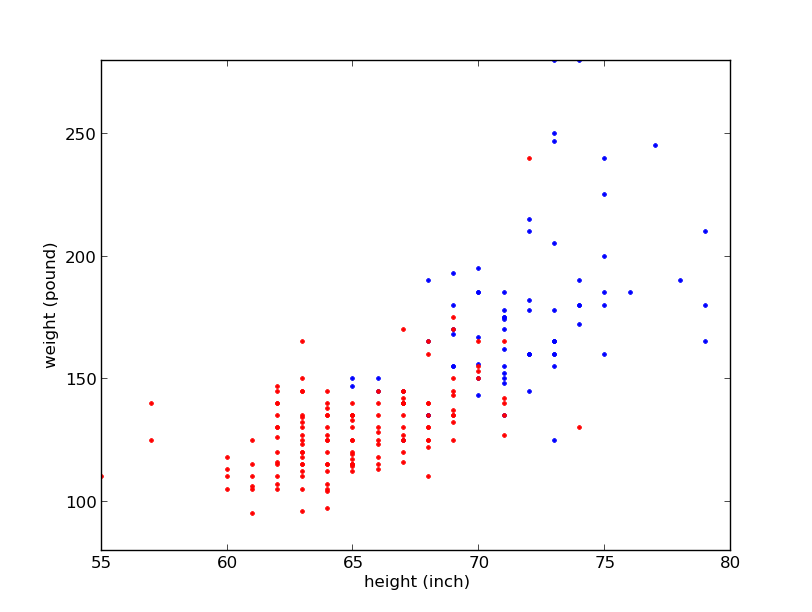
\includegraphics[height=6cm]{plotbio.png}


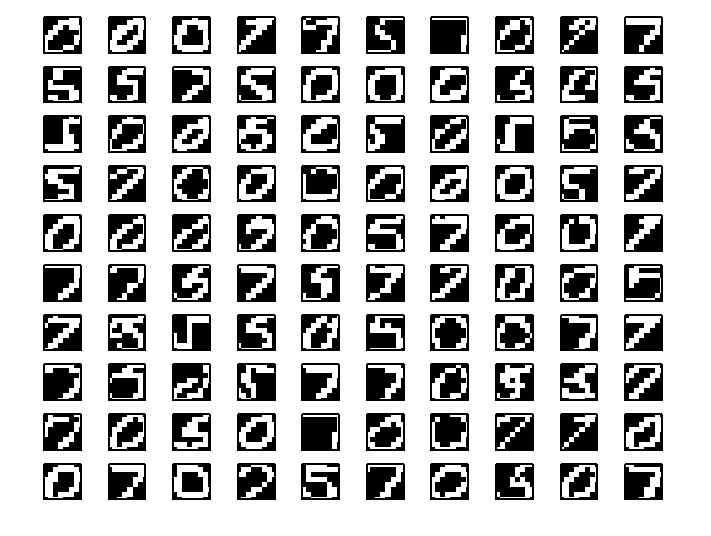
\includegraphics[height=6cm]{digits.png}




\end{document}
